\documentclass[a4paper,11pt]{article}

%%% Работа с русским языком
\usepackage{cmap}					% поиск в PDF
\usepackage{mathtext} 				% русские буквы в формулах
\usepackage[T2A]{fontenc}			% кодировка
\usepackage[utf8]{inputenc}			% кодировка исходного текста
\usepackage[english,russian]{babel}	% локализация и переносы

\usepackage[a4paper,left=3cm,right=2.5cm,top=2.5cm,bottom=2.5cm]{geometry}

%%% Дополнительная работа с математикой
\usepackage{amsmath,amsfonts,amssymb,amsthm,mathtools} % AMS
\usepackage{icomma} % "Умная" запятая: $0,2$ --- число, $0, 2$ --- перечисление

%%% Программирование
\usepackage{etoolbox} % логические операторы

% https://tex.stackexchange.com/questions/60545/should-i-mathrm-the-d-in-my-integrals#60546
\newcommand*\dif{\mathop{}\!\mathrm{d}}

%%% Запрет на перенос строк в формулах
\binoppenalty=10000  % разрывы строк после знаков бинарных операций (+ - * итд)
\relpenalty=10000    % разрывы строк после знаков бинарных отношений (= > < итд)

\usepackage{setspace}
%\onehalfspacing        % полуторный интервал для всего текста

% https://tex.stackexchange.com/questions/59245/how-to-disable-automatic-indent#59248
\usepackage{parskip}

%%% Работа с картинками
\usepackage{graphicx}  % Для вставки рисунков
\graphicspath{{images/}}  % папки с картинками
\setlength\fboxsep{2pt} % Отступ рамки \fbox{} от рисунка
\setlength\fboxrule{1pt} % Толщина линий рамки \fbox{}
\usepackage{wrapfig} % Обтекание рисунков и таблиц текстом

%% make vectors bold
\renewcommand{\vec}[1]{\mathbf{#1}}

\usepackage{hyperref}
\hypersetup{colorlinks=true,urlcolor=blue}

%%% Заголовок
\title{ML From Data}
\author{}
\date{}

%%% конец преамбулы, начало документа
\begin{document}

\maketitle

\url{https://courses.edx.org/courses/course-v1:CaltechX+CS1156x+3T2017/course/}



\section{Week \#1}

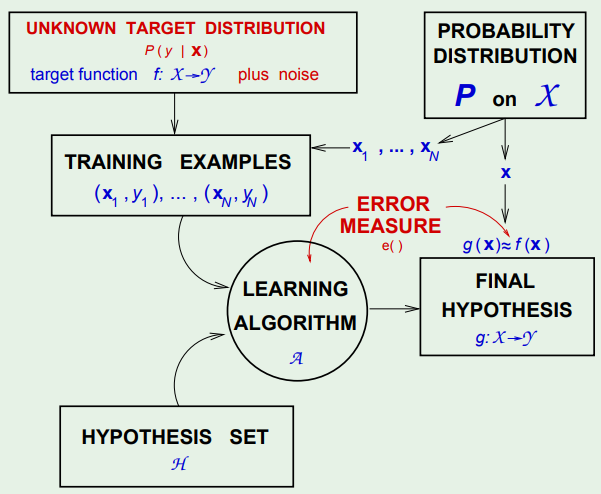
\includegraphics[scale=.66]{structure.png}

Good generalization: $E_{in}(g) \approx E_{out}(g)$

Learning: $g \approx f$  $\Longleftrightarrow$  $E_{out}(g) \approx 0$

\textellipsis



\section{Week \#2}

\def\iiside{\; \rule[.5ex]{2.0em}{0.2pt} \;}
\def\iicode#1{\texttt{#1}}

\def\iiEin{E_{in}}
\def\iiEout{E_{out}}
\def\iiE{\mathbb{E}}
\def\iiD{\mathcal{D}}
\def\iiH{\mathcal{H}}
\def\iiX{\mathcal{X}}
\def\iiw{\vec{w}}
\def\iix{\vec{x}}
\def\iiy{\vec{y}}

$ X = \begin{bmatrix}
        \iiside \vec{x}_1^T \iiside \\
        \iiside \vec{x}_2^T \iiside \\
                 \vdots             \\
        \iiside \vec{x}_N^T \iiside
      \end{bmatrix} $
--- input data matrix,
$ \vec{y} = \begin{bmatrix} y_1 \\ y_2 \\ \vdots \\ y_N \end{bmatrix} $
--- target vector

\[ \iiEin(\iiw) = \frac{1}{N} \left\| X \iiw - \iiy \right\|^2 \]

\[ \nabla \iiEin(\iiw) = \frac{2}{N} X^T (X \iiw - \iiy) = \vec{0} \]

\[ \iiw = X^\dagger \iiy  \quad \text{where} \quad  X^\dagger = (X^T X)^{-1} X^T \]

$X^\dagger$ --- pseudo-inverse, \iicode{numpy.linalg.pinv(X)}

\subsection{Error Measure}

\[ \iiEin = \frac{1}{N} \sum_{n=1}^{N} e\left(h(x_n),f(x_n)\right) \]

\[ \iiEout = \iiE_{\iix}\left[ e\left(h(\iix),f(\iix)\right) \right]  \]

\subsection{Noisy Targets}

Instead of $y=f(\iix)$ we use target \emph{distribution}: $ P(y|\iix) $

$(\iix,y)$ is now generated by joint distribution: $ P(x) P(y|\iix) $

Noisy target $\equiv$ deterministic target $f(x) = \iiE(y|\iix)$
$\; \pm$ some noise $\left( y - f(\iix) \right)$



\section{Week 3}

\subsection{Theory of generalization}

\def\iimH{m_\iiH}

\href{https://en.wikipedia.org/wiki/Hoeffding%27s_inequality}{Hoeffding's} inequality:
\[ P\left[|\iiEin(g) - \iiEout(g)| > \epsilon \right] \leqslant 2Me^{-2 \epsilon^2 N} \]

This inequality is a form of the large numbers law.
The statement $\iiEin=\iiEout$ is \emph{PAC} (probably approximately correct).

$M$ -- number of functions in the hypothesis set $\iiH$,
$N$ -- number of \emph{dichotomy} points

\[ \iimH(N) = \max_{\iix_1,\dots,\iix_N\in\iiX}
                    \left| \iiH(\iix_1,\dots,\iix_N) \right|
   \quad\text{--- growth function} \]

When you get all possible hypotheses, all possible dichotomies,
you say that the hypothesis set $\iiH$ \emph{shattered} the points --
broke them in all possible $2^N$ ways.

$k$ --- \emph{break point}, minimum $N$, where number of dichotomies cannot reach $2^N$

If $k=\infty$ (no break point), then $\iimH(N) = 2^N$

$B(N,k)$ --- maximum number of dichotomies on $N$ points, with break point $k$

\[ B(N,k) \leq \alpha+2\beta = (\alpha+\beta) + \beta = B(N-1,k) + B(N-1,k-1) \quad\ldots \]

\[ B(N,k) = \sum_{i=0}^{k-1} \binom{N}{i} \]

\[ \text{Note:}\quad
   \binom{n}{k} = \frac{n!}{k!(n-k)!}
   = \frac{1}{k!} \underbracket{ n(n-1)\cdots(n-k+1) }_{k\text{ times}} \sim n^k \]

\[ \iimH(N) \leqslant B(N,k) = \sum_{i=0}^{k-1} \binom{N}{i} \sim N^{k-1}
   \quad\text{--- polynomial} \]

Note: order of the polynomial depends on the break point.

The \href{https://en.wikipedia.org/wiki/Vapnik%E2%80%93Chervonenkis_theory}{Vapnik-Chernovenskis} inequality:

\[ P \big[\, |\iiEin(g) - \iiEout(g)| > \varepsilon \,\big] \leqslant
   4 \iimH(2N) \, \scalebox{1.4}{$ e^{-\frac18 \varepsilon^2 N} $}
   \; (\triangleq \delta) \]



\section{Week 4}

\subsection{VC dimensions}

\def\iidvc{d_{VC}}

The VC dimension $\iidvc(\iiH)$ is the the most points $\iiH$ can shatter.

\[ \iimH(N) \leq \sum_{i=0}^{d_{VC}} \binom{N}{i} \sim N^{d_{VC}} \]

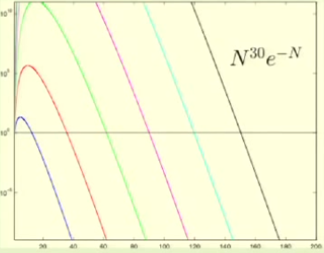
\includegraphics[scale=1]{plot_n^d_e^-n.png}

\[ \text{Rule of thumb:}\quad P \lesssim 10^{-1} \Longleftrightarrow N \gtrsim 10 d_{VC} \]

\[ \text{(probability bound)} \;
   \delta = 4 \, \iimH(2N) \, \scalebox{1.4}{$ e^{-\frac18 \epsilon^2 N} $}
   \Longleftrightarrow
   \epsilon = \sqrt{ \frac{8}{N} \ln{ \frac{ 4 \, \iimH(2N) }{\delta} } }
   \; (\triangleq \Omega) \]

With probability $P = 1 - \delta$, $\left| \iiEout - \iiEin \right| \leq \Omega(N,\iiH,\delta)$

Generalization bound: \[ \iiEout \leq \iiEin + \Omega \]

\[ |\iiH| \!\uparrow \; \Rightarrow \iiEin \!\downarrow \;\text{ but }\; \Omega \!\uparrow  \]

\subsection{Bias-Variance Tradeoff}

\def\iiD{\mathcal{D}}
\def\iiE{\mathbb{E}}
\def\iix{\vec{x}}
\def\iiEx{\iiE_\iix}
\def\iiED{\iiE_\iiD}
\def\iifx{f(\iix)}
\def\iigDx{g^{(\iiD)}(\iix)}
\def\iigBarx{\bar{g}(\iix)}
\def\iivar{\mathbf{var}}
\def\iibias{\mathbf{bias}}

\[ \iiEout(\iiD) = \iiEx \left[ \left( \iigDx - \iifx \right)^2 \right] \]

Average hypothesis: \[ \iigBarx = \iiED \left[ \iigDx \right] \]

\[ \iiED \left[ \left( \iigDx - \iifx \right)^2 \right] =
   \underbracket{ \iiED \left[ \left( \iigDx - \iigBarx \right)^2 \right] }_{ \iivar(\iix) }
   + \underbracket{ \big( \iigBarx - \iifx \big)^2 }_{ \iibias(\iix) } \]

\[ \iibias = \iiEx \left[ \big( \iigBarx - \iifx \big)^2 \right] \]

\[ \iivar = \iiEx \left[ \iiED \left[ \left( \iigDx - \iigBarx \right)^2 \right] \right] \]



\end{document}
